%%% -*-LaTeX-*-
\chapter{Time scale of very large scale motions}\label{chap:chap3}
Dynamic Mode Decomposition (DMD) has been used to study the time scale of Very Large Scale Motions (VLSMs) in the atmospheric boundary layers. While the length scales of VLSMs have been identified in previous studies, the time scale of evolution has not been identified objectively. It was reported in the earlier studies that VLSMs convect with a velocity lower than the local mean velocity. The time scales of VLSMs were found to be much larger than the large eddy turnover time, which is in line with the previous findings. DMD results also show that low-momentum and high-momentum regions appear alternatively in the spanwise direction as was observed from experiments and other visualization methods. However, the spanwise extent of the VLSMs appears to be significantly lower than what was estimated by earlier studies.


\section{Introduction}
Understanding the hierarchy of scales and how these scales interact is fundamental towards understanding  turbulent flow phenomena and devising mechanisms to control turbulent mixing processes. A common line of inquiry is to examine the spatial organization of turbulent motions at different scales using flow visualization technique. Typically, a visualization experiment is carried out using a passive scalar as a tracer. Such experiments can reveal the presence of multiple hierarchical scales and their relative motions. For example, a silhouette image of a large-scale structure resulting from the conglomeration of finer scale motions has been captured in  Boundary Layer (BL) flows \citep{falco_pof_77, hommema_adrian_blm_03}. These visualization experiments by \citet{falco_pof_77} and \citet{hommema_adrian_blm_03} provided insight on the organization of large-scale motions in the BL including the visual identification of inclined ramp like structures previously identified. However, \citet{hussain_1986_jfm} discussed caveats of visualisation technique and emphasizes that caution must be taken in interpretation of scalar marked boundary lines of structures. Still, when a sufficient description of the flow field is available from a simulation or experiment, data driven modeling can be used as a surrogate of the experimental methods while avoiding some of the limitations of experimental methods. One of the convincing qualities of data-driven methods is that they  do not heavily depend on the use of subjective parameters as used in conventional conditional averaging. Among the data-driven techniques, mainly two methods, i.e., Proper Orthogonal Decomposition (POD) \citep[eg., ][]{li_bouzeid_blm_2011,muld_compFluids_2012} and Dynamic Mode Decomposition (DMD). \citep[eg., ][]{bagheri_jfm2013,liu_ExpF_2015,muld_compFluids_2012} have been used widely. \citet{taira_arxiv_2017} summarized the most important strengths and weaknesses of both methods. 

A general strategy of studying flow structures is to project velocity fields on to different basis vectors i.e., Fourier modes, empirical eigen vectors, and discrete wavelet basis vectors. The velocity field is usually decomposed as a linear combination of orthogonal basis functions at a given time as $u(\mathbf{x},t) = \sum_k a_k \phi_k(\mathbf{x},t)$ where $\phi_k(\mathbf{x})$ represents the basis vectors and $a_k$ represents coefficients of the projections. Alternatively, it is possible to decompose the velocity field into a fixed set of orthogonal spatial functions with time-dependent projection coefficients,  i.e., $u(\mathbf{x},t)=\sum_k a_k(t) \phi_k(\mathbf{x})$  where $u(\mathbf{x},t)$ denotes a velocity field, $a_k(t)$ denotes the time-dependent  coefficients of projection, and $\phi_k(\mathbf{x})$ denotes orthogonal spatial functions capturing the spatial description of the field \citep{taira_arxiv_2017}. Such a decomposition underpins the Galerkin projection schemes used in computational fluid dynamics \citep{rowley2004model, armbruster_chaos_94} and form the basis of  the Proper orthogonal Decomposition (POD), which is a common tool to identify the spatial structures of energetic scales in a turbulent flow and has been used to study the spatial structure of Very Large Scale Motions (VLSMs) \citep[][]{Hellstrom_pof_2011,bailey_smits_jfm_2010}. However, to study the temporal evolution of motions at any scale, a POD based gelarkin projection scheme must be adopted to determine the time dependent expansion coefficients. A POD basis is extracted from a full-scale simulation and then the system is modeled on a reduced set of the POD bases. Next, proper boundary and initial conditions for the new basis are set before solving the resultant system of ordinary differential equations in order to determine the time-dependent expansion coefficients ($a_k(t)$) \citep[eg,. ][]{stabile2017advances}. If only the spatial structure coherent motions is of interest, determining the spatial basis vectors $\phi_k(\mathbf{x})$ is sufficient. Many studies have used POD to this end \citep[eg., ][]{li_bouzeid_blm_2011,muld_compFluids_2012}. 

The relatively new method of modal decomposition, namely Dynamic Mode Decomposition (DMD), is advantageous in short time flow evolution studies. DMD is completely data driven and does not require any knowledge of the underlying conservation laws that govern the dynamics, unlike POD method. Another attractive feature of DMD is that it can isolate dynamic structures with a particular frequencies where POD modes can correspond to a mix of frequencies. This feature makes DMD useful to isolate and rank structures that evolve at different time scales and study their spatial patterns. DMD have been successfully used to identify structures behind bluff bodies, but has so far not been used to characterize VLSMs in the high Reynold's number boundary layer where the only restriction on scale separation is the dynamic range of the simulation and experimental data in contrast to finite Reynold's number direct numerical simulation studies.  In this study, DMD is used to study the spatial and temporal characteristics of VLSMs in the atmospheric boundary layers under two different forcing conditions. 

\section{Large Eddy Simulation}
Large Eddy Simulation (LES) was carried out to simulate an Ekman layer and flow in a channel. Resolution in horizontal and vertical directions were $62.5\ m$ and $7.89\ m$, respectively. The same numerical LES code along with the same subgrid-scale model that was used to study VLSM characteristics in Chapters \ref{chap:chap1} and \ref{chap:chap2} has been used to generate the flow fields (see Sec. \ref{sec:num_sim_chap_1} and \ref{sec:LES_chap2} ). However, to keep the computational cost of the DMD analysis within a reasonable limit, grid points in horizontal directions were reduced to 768 and in the vertical direction, a total of 96 grid points. The flow domain spanned $48$ Km in the horizontal ($x$, $y$) directions and 750.0 m in the wall-normal direction ($z$) for $EK02$ and 1500.0 m for $CHNL$. The parameters of the simulations are shown in Table \ref{tab:sim_param}. The reduced domain size here should not pose any limitations to the evolution of VLSMs because the results in Chapter \ref{chap:chap1} confirms that the maximum length scale of VLSMs is no larger than $25\delta$.

%An analysis of 8000 instantaneous two dimensional frames of u-velocity component required analysing a data matrix of 37.74 gigabyte. %A decomposition of the full three dimensional u-component of the velocity field into DMD modes would require operations to be carried over a data matrix of size 3.62 terabyte. 


\section{Dynamic Mode Decomposition} DMD can be applied to experimental and numerical data sets alike. This analysis provides dynamic modes that evolve with certain frequencies and are associated with a decay or growth rate. The dynamic modes are composed of recognizable spatial patterns that can be interpreted as organizational units of fluid flow fields or loosely as eddies. The DMD method approximates the state of a system, e.g., as a component of the velocity field, $u \in R^{N}$ from one time instance ($m$) to another ($m+1$) with the Koopman operator $A$ as
\begin{align}
u_{m+1}= A u_{m}\ .
\label{eqn:iterative_reln}
\end{align}
An ensemble of $M$ snapshots of $u$ obtained with a fixed time interval $\Delta t$ between snapshots can be organized in two matrices $X$ and $Y$
\begin{align}
X & = [u_{1}\ u_{2} \ \cdots \ u_{M-1}], \\
Y & = [u_{2}\ u_{3} \ \cdots \ u_{M}]\ ,
\end{align}
which using Eqn. \ref{eqn:iterative_reln} can be rewritten as
\begin{align}
X & = [u_{1}\ Au_{1} \ \cdots \ A^{M-2}u_{1}] \label{eqn:X_approx}, \\
Y & = [Au_{1}\ A^{2}u_{1} \ \cdots \ A^{M-1}u_{1}] \label{eqn:Y_approx}. 
\end{align}
The columns of $X$ and $Y$ are each elements of a Krylov subspace and the last vector in $Y$ can be approximated within the span of the Krylov subspace in an $L^{2}$ sense \citep{kutz_book2013} as
\begin{align}
u_{M} = \sum_{i=1}^{M-1}b_{i} u_{i}+ r,
\label{eqn:last_vec_approx}
\end{align}
where $b_i$ are the coefficients of the Krylov space vectors and $r$ is the residual. Schmid \citep{schmid_jfm2010} suggests that after a critical number of snapshots, adding more snapshots in $X$ or $Y$, i.e., any more columns, would not improve the vector space spanned by $X$ and at this point, the last data vector approximation (Eqn. \ref{eqn:last_vec_approx}) would not improve any more. This could practically serve as a limit to the number of snapshots used in calculation. Up until this point, the Koopman operator $A$ is unknown. The key idea of DMD is to find an approximation to the eigen vectors and eigen values of $A$. From \ref{eqn:X_approx} and \ref{eqn:Y_approx}, a transformation relationship between $X$ and $Y$ can be expressed as
\begin{align}
 Y = A X.
\label{eqn: y=ax}
\end{align}
This matrix equation can also be rewritten following Eqn. \ref{eqn:last_vec_approx} as
\begin{align}
  Y =X S + r e^{T}_{M-1},
\end{align}
where $e_{M-1} \in R^{(M-1) \times 1}$ is the $(M-1)$th unit vector, $r \in R^{N \times 1}$, and $S \in R^{N \times (M-1)}$ is a matrix of the companion type and assumes the form
\begin{align}
S =
    \begin{bmatrix}
        0 & \cdots &        & 0  & b_1\\
        1 & \ddots &        & 0  & b_2 \\
        0 & \ddots & \ddots &    & \vdots \\
          & \ddots & \ddots & 0  & b_{M-2} \\
        0 & \cdots & 0      & 1  & b_{M-1}
    \end{bmatrix}\ .
\end{align}
The last column of $S$ contains the unknown coefficients of Eqn. \ref{eqn:last_vec_approx}. Eigen values of $S$ approximate some of the eigen values of $A$. However, calculating matrix $S$ requires the operator $A$ to be known to proceed with an Arnoldi algorithm. \citet{schmid_jfm2010} suggested calculating a matrix $\tilde{S}$ instead of $S$, where $\tilde{S}$ is a similar matrix to $A$. Utilizing reduced singular value decomposition of the data matrix $X$ and following Eqn. \ref{eqn: y=ax}, $\tilde{S}$ can be calculated from
\begin{align}
U^{*} A U  = U^{*} YW  \Sigma^{-1} \equiv \tilde{S},
\end{align}
where $X=U\Sigma W^{*}$. At this point, the following eigen value problem is solved,
\begin{align}
\tilde{S}y_{k}  =  \mu_{k} y_{k} 
\end{align}
where the eigen values $\mu_{k}$ capture the time dynamics of the discrete Koopman operator $A$ \citep{kutz_book2013}. DMD modes $\phi_{k}$ are obtained when the eigen vectors $y_{k}$ are projected to the reduced column space of $X$ as
\begin{align}
\phi_{k} = Uy_{k}.
\end{align}
The future state of the flow field at any time $n \Delta t$ can be predicted from DMD modes, 
\begin{align}
x_{n} = \sum_{k=1}^{K} b_{k} \phi_{k}(x) \text{exp}(\omega_{k} t),
\end{align}
or in matrix form, 
\begin{align}
x_{DMD}(t)= \Phi\  \text{diag}(\text{exp}(\omega t)) b,
\end{align}
where $\omega_k = \ln (\mu_{k})/ \Delta t$, $\Phi$ is a matrix whose columns are the eigen vectors $y_{k} $ and $b_{k}$ are the initial amplitudes of each mode. The $b_{k}$ amplitudes are obtained from the equation, $x_1=\Phi b$, using Moore-Penrose pseudo-inverse $\Phi^{+}$ such that,
\begin{equation}
 b = \Phi^{+}x_{1} .
\end{equation}
The algorithm as has been described was first proposed by \citet{schmid_jfm2010} and a more elaborate version can be found in \citep{kutz_book2013, rowley_mezic_schlatter_jfm_2009,tu_thesis}. This is the most widely used DMD algorithm, although a proliferation of modified DMD algorithms exists that have been observed to have a finer separation of multiscale spatio-temporal features \citep[eg., ][]{kutz_fu_brunton_siam_2016}, can handle data sampled at irregular time intervals \citep[][]{tu_thesis}, can apply DMD to spatially sub-sampled data \citep{florimond_mathelin_pof_2015}, and can manage large and streaming datasets \citep{hemati_pof_2014}.

Following the algorithm as has been described, DMD was carried out over 8000 frames for both the cases. For $CHNL$, the constant time spacing between consecutive frames ($\Delta t$) was $0.1$ sec. and for $EK02$, it was $2$ sec. Since three dimensional DMD analysis is prohibitively expensive in terms of requirement of the Random Access Memory, two-dimensional DMD was carried out on wall parallel and spanwise-vertical planes. Data were extracted at a particular streamwise-spanwise plane from the three dimensional velocity field for all the 8000 time instances and were stacked as columns in the data matrices $X$ and $Y$ to proceed with DMD mode extraction. Each of the matrices  $X$ and $Y$ required $37.7\ GB$ of memory. In case of full 3D analysis, the matrix size will rise to $3623.8\ GB$. 

\section{Results and Discussion}
DMD separates spatial structures that have different frequencies. Here, the frequency distribution of DMD modes at different heights was examined for both cases. A series of 8000 frames that were equally spaced in time scale was analyzed resulting in 8000 DMD modes that were sorted based on frequency ($\mu_k$). Modes having zero frequency were excluded from analysis because these modes would constitute the mean flow field. Time periods of 5-10 representative DMD modes are categorized against normalized height in Table \ref{tab:dmd_freq_chnl} for $CHNL$ and in Table \ref{tab:dmd_freq_ek02} for $EK02$. DMD time periods ($\Delta T$) are the inverse of the pure sine or cosine frequencies that correspond to the DMD eigen values and they are normalized with large length and velocity scales ($\Delta T / (\delta/U(\delta))$) where ($\delta/U(\delta)$) constitutes large eddy turnover time where and $U(\delta)$ is the mean velocity at the top of the boundary layer. Differences between frequencies of the first few modes resolved at different heights are observed, although for any particular mode,  discernible trends with height are not observed. Spatial structures corresponding to DMD modes are shown in Figs. \ref{fig:chnl_dmd_modes_z_4_7} and \ref{fig:ek02_dmd_modes_z_4_24}. To characterise length scales of LSMs and VLSMs comprised of low-speed fluid, velocity fields were reconstructed from the individual DMD modes at selected heights to be utilized in the structure detection procedure. To identify structures of different length scales an alternative definition adopted in Chap. \ref{chap:chap1} was used, i.e., a connected region of low-speed fluid in the binarized flow field. In case of $CHNL$, DMD modes with normalized time periods of 12.91, 6.76, 5.75, 4.74 as categorically presented against normalized height of $0.50\delta$ in Table \ref{tab:dmd_freq_chnl} were analysed.  In case of $EK02$, the DMD modes with normalized time periods of 136.5, 37.65, 21.86, 15.17 at a height of $0.48\delta$ were selected. The key observation that emerges from Fig. \ref{fig:dmd_length_scale_dist} is that contrary to primary expectation, a particular DMD mode does not isolate a single length scale. Any DMD mode is observed to comprise a distribution of length scales. So, while DMD modes can perfectly isolate dynamics based on time scale, the isolation of coherent spatial structure may not be clean. 

From the results, it is also apparent that structures that evolve over a very long time scale can be obtained in both the log and wake layers. Since a linear proportionality between the time scale and the length scale can be established following Taylor's frozen turbulence hypothesis, it can be inferred that the DMD modes with long time period would correspond to long length scales. However, an observation Fig. \ref{fig:dmd_length_scale_dist} suggests otherwise. Fig. \ref{fig:dmd_length_scale_dist}(a) shows the normalized histogram of the size distribution of the structures in the reconstructed velocity field for the $CHNL$ and Fig. \ref{fig:dmd_length_scale_dist}(b) shows the same for $EK02$. A limit in the length scale of the identified structures is observed, e.g., for $Ek02$ the maximum identified normalized length scale is $15$, whereas the normalized DMD time scale is $37.4$. 

DMD is sensitive to the sampling frequency and follows Nyquit-Shannon sampling theorem. For the $CHNL$ case, sample velocity fields were collected every 0.1 sec and for $Ek02$, the sampling rate was 2 sec. Therefore, for $CHNL$, any process that evolves with a time period of less than 0.2 sec would not be captured by the DMD decomposition and for $EK02$, that time period would be any less than 4 sec. Since this study is concerned with LSMs and VLSMs that are presumed to correspond with very long time scales, these sampling frequencies should be sufficient. The ratio between the sampling rate of $Ek02$ and $CHNL$ is 20. This difference is reflected in the obtained time periods of DMD modes. A comparison between Tables \ref{tab:dmd_freq_chnl} and \ref{tab:dmd_freq_ek02} show that the time period of the first first few modes of $EK02$ can be as large as 11 times larger than that of $CHNL$. However, in $EK02$, the DMD modes that appeared with very large time periods do not show any coherent motions that corresponds to the expected shape or length scales of VLSMs or LSMs. For example, DMD mode with characteristic normalized time scales of 136.50, 37.65, 21.86 as portrayed in Fig.  \ref{fig:ek02_dmd_modes_z_4_24} show less prominence of VLSMs as is apparent from Fig.  \ref{fig:dmd_length_scale_dist}(b), which shows the distribution of length scales. These modes that correspond to very large time periods that also do not show recognizable coherence in the plots will most likely appear as zero modes if sampling period was lower. 

An overall observation from the Tables \ref{tab:dmd_freq_chnl} and \ref{tab:dmd_freq_ek02} and plots in Fig. \ref{fig:dmd_length_scale_dist} is that VLSMs persist for a long period of time compared to their length scale. The existence of smaller scale motions are also observed in the scale distribution of slow DMD modes as shown in Fig. \ref{fig:dmd_length_scale_dist}. 

\section{Summary and Conclusions}
Large eddy simulations were carried out to study the structure of VLSMs in a pressure-driven channel flow and in an Ekman layer flow. Eight thousand successive frames were recorded from the simulation to investigate the time and length scale of VLSMs using the DMD method. DMD method produced constituent DMD modes that correspond to individual frequencies and could project the temporal evolution of the velocity field over a period of time. The spatial pattern of the individual DMD modes corresponding to a range of frequencies within the time scale of interest were investigated to understand the spatial structure of the VLSMs. It was observed that while DMD method could isolate modes evolving under different frequencies, the spatial patterns were not distinctively unique for any of the modes. Using image processing techniques and under the assumption that connected regions on a thresholded velocity field constitute coherent structures, the reconstructed velocity fields from DMD modes were analysed. It was observed that each DMD mode contained various length scales. The results showed that within the spatial structure of any DMD mode, LSMs were dominant in numbers and the existence of VLSMs with length scales greater than $10\delta$ was rare. The results also indicated that VLSMs and LSMs can evolve over a longer time scale compared to their expected advection time scale estimated from Taylor's frozen turbulent hypothesis. 

\bibliographystyle{unsrtnat}
\bibliography{MyThesisRefs}
\clearpage
 
 %% =================== all tables ========================

    \begin{table}
    \caption{Simulation parameters}
    \centering
	\begin{tabular}{ c c c c c c c c}
	\hline 
		       & $N_1/N_2$ & $N_3$   & $L_1/L_2$(Km)  & $L_3$ (Km) & $\delta$(m)   & $Ro$ \\
    \hline 
     $EK02$    & 768       &  96     & 48             &  0.75      & 563           & 33  \\
     $CHNL$    & 768       &  96     & 48             &  1.5       & 1500          & - \\
    \hline 
    \hline 
    \end{tabular}
    \label{tab:sim_param}
    \end{table}

\begin{table}
\caption{Time period of evolution of the first five DMD modes normalized by $\delta / U(z)$ for $CHNL$. Modes were calculated at different horizontal planes characterized by normalized heights presented.}
  \begin{center}
  \begin{tabular}{  c  c c c c c  } 
  \hline
  \hline
  Normalized Height & Mode 1 & Mode 2 & Mode 3 & Mode 4 & Mode 5          \\

  \multirow{1}{4em}{$0.047\delta$}  & 27.09 & 10.19 & 6.11 & 4.63 & 3.48  \\
  \hline
  \multirow{1}{4em}{$0.095\delta$}  & 14.05 & 8.78  & 5.65 & 4.07 & 3.16  \\
  \hline
  \multirow{1}{4em}{$0.2\delta$}    & 32.07 & 11.68 & 6.49 & 5.01 & 3.75  \\
  \hline
  \multirow{1}{4em}{$0.33\delta$}   & 50.59 & 12.87 & 7.22 & 4.93 & 3.94  \\
  \hline 
  \multirow{1}{4em}{$0.50\delta$}   & 12.91 & 6.76  & 5.75 & 4.74 & 3.70  \\
  \hline
  \hline
  \end{tabular}
  \end{center}
\label{tab:dmd_freq_chnl}
\end{table}

\begin{table}
\caption{Statistics of the first five DMD modes for $EK02$. DMD time periods are normalized by $\delta / U(z)$. Modes were calculated at different horizontal planes characterized by normalized heights presented.}
\begin{center}
\small
\begin{tabular}{  c c c c c c c} 
\hline
\hline  
Normalized Height  & Mode 1 & Mode 2 & Mode 3 & Mode 4 & Mode 5  \\

\multirow{1}{4em}{$0.04\delta$}  & 115.5 & 38.6 & 22.4 & 15.4 & 11.7  \\
\hline
\multirow{1}{4em}{$0.21\delta$}  & 113.4 & 34.8 & 20.4 & 14.7 & 11.4  \\ 
\hline
\multirow{1}{4em}{$0.32\delta$} & 100.2  & 35.6 & 20.8 & 14.7 & 11.4  \\ 
\hline
\multirow{1}{4em}{$0.48\delta$} & 135.7  & 37.4 & 21.7 & 15.0 & 11.6  \\ 

\end{tabular}
\begin{tabular}{  c c c c c c} 
\hline
Normalized Height  & Mode 6 & Mode 7 & Mode 8 & Mode 9 & Mode 10 \\

\multirow{1}{4em}{$0.04\delta$} & 9.6 & 8.1 & 7.5 & 7.0 & 6.2  \\
\hline
\multirow{1}{4em}{$0.21\delta$}  & 9.5 & 8.1 & 7.1 & 6.2 & 5.5  \\ 
\hline
\multirow{1}{4em}{$0.32\delta$}  & 9.4 & 7.9 & 7.1 & 6.2 & 5.5   \\ 
\hline
\multirow{1}{4em}{$0.48\delta$}  & 9.5 & 8.0 & 7.1 & 6.2 & 5.5   \\ 
\hline
\hline
\end{tabular}
\end{center}
\label{tab:dmd_freq_ek02}
\end{table}


%%===================== all figures =======================

\graphicspath{{chap3Img/}}
\begin{figure}[htb]
	\begin{minipage}{\textwidth}
	\setlength{\unitlength}{1in}
	  \begin{picture}(6,3)
		\put(0,0){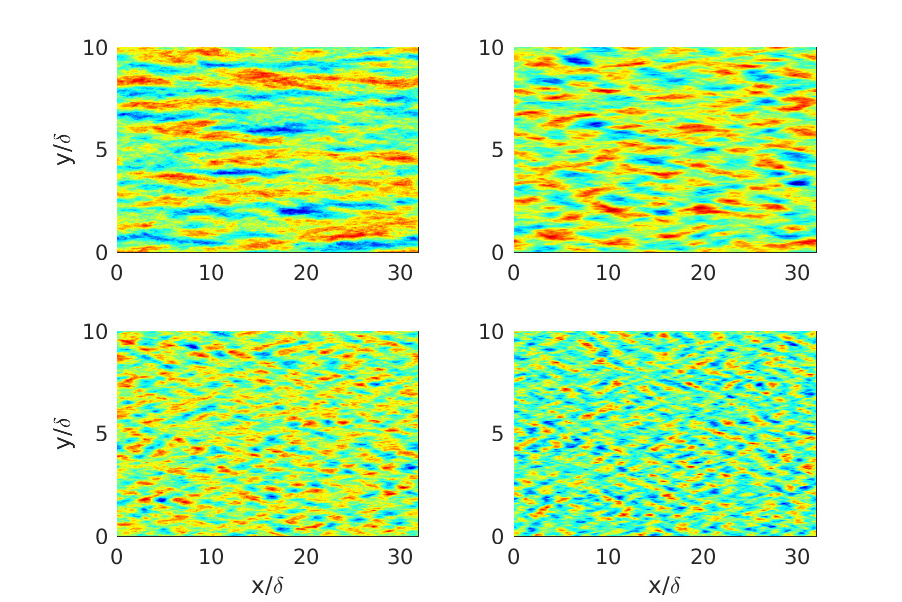
\includegraphics[width=6.0in,height=3in]{chnl_dmd_4mode_z_4-eps-converted-to}}
		\put(-0.1,2.5){$\mathbf{(a)}$}
		\put(1.6,0.05){\colorbox{white}{\makebox(0.5,0.05){$x/\delta$}}}
		\put(4.0,0.05){\colorbox{white}{\makebox(0.5,0.05){$x/\delta$}}}
		\put(0.25,0.7){\colorbox{white}{\makebox(0.2,0.25){$y/\delta$}}}
		\put(0.25,2.2){\colorbox{white}{\makebox(0.2,0.25){$y/\delta$}}}
	  \end{picture}
	\end{minipage}

	\begin{minipage}{\textwidth}
	\setlength{\unitlength}{1in}
	\begin{picture}(6,3)
		\put(0,0){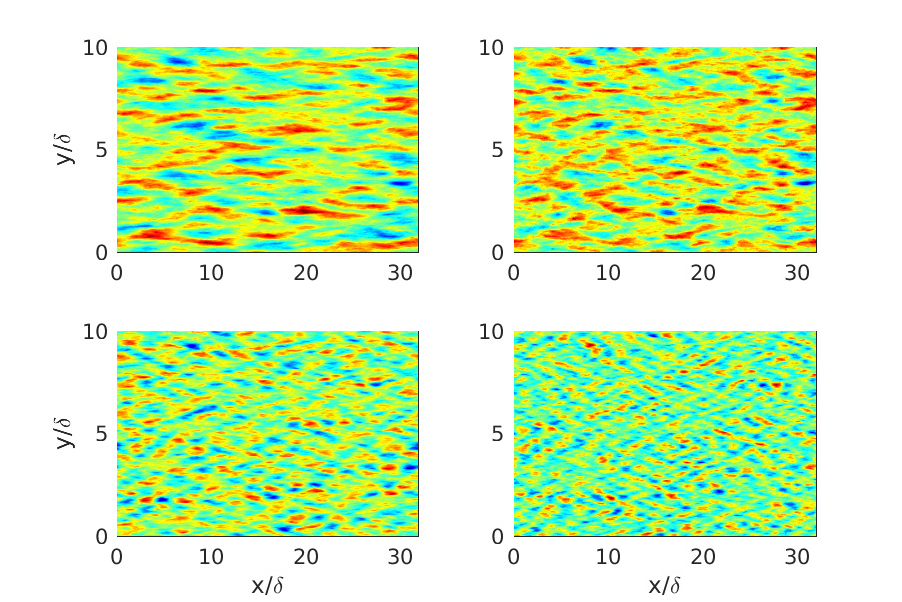
\includegraphics[width=6.0in,height=3.0in]{chnl_dmd_4mode_z_7-eps-converted-to}}
		\put(-0.1,2.5){$\mathbf{(b)}$}
		\put(1.6,0.05){\colorbox{white}{\makebox(0.5,0.05){$x/\delta$}}}
		\put(4.0,0.05){\colorbox{white}{\makebox(0.5,0.05){$x/\delta$}}}
		\put(0.25,0.7){\colorbox{white}{\makebox(0.2,0.25){$y/\delta$}}}
		\put(0.25,2.2){\colorbox{white}{\makebox(0.2,0.25){$y/\delta$}}}		
	\end{picture}
	\end{minipage}
\caption{First four DMD modes with characteristic time period as listed in Table \ref{tab:dmd_freq_chnl} at heights $0.047\delta$ and $0.095\delta$ for the $CHNL$ case are shown in subfigure (a) and (b), respectively. In subfigure (a), top left panel shows spatial mode corresponding to normalized time period ($\Delta T U(\delta)/ \delta$) of 27.09 and top right, bottom left, bottom right panels correspond to 10.19, 6.11, 4.63, respectively. In subfigure (b) panels beginning from top left corner in the clockwise order corresponds to normalized time periods 14.05, 8.78, 5.65, and 4.07, respectively.}
\label{fig:chnl_dmd_modes_z_4_7}
\end{figure}

\graphicspath{{chap3Img/}}
\begin{figure}[htb]
	\begin{minipage}{\textwidth}
	\setlength{\unitlength}{1in}
	  \begin{picture}(6,3)
		\put(0,0){\includegraphics[width=6.0in,height=3in]{ek02_dmd_mode-1-4_z_24_unstable}}
		\put(-0.1,2.5){$\mathbf{(a)}$}
		\put(1.5,0.00){\colorbox{white}{\makebox(0.5,0.05){$x/\delta$}}}
		\put(4.5,0.00){\colorbox{white}{\makebox(0.5,0.05){$x/\delta$}}}
		\put(-.05,0.60){\colorbox{white}{\makebox(0.2,0.25){$y/\delta$}}}
		\put(-.05,2.2){\colorbox{white}{\makebox(0.2,0.25){$y/\delta$}}}
	  \end{picture}
	\end{minipage}

	\begin{minipage}{\textwidth}
	\setlength{\unitlength}{1in}
	\begin{picture}(6,3)
		\put(0,-0.05){\includegraphics[width=6.0in,height=3.0in]{ek02_dmd_mode-5-8_z_24_unstable}}
		\put(-0.1,2.5){$\mathbf{(b)}$}
		\put(1.5,-0.05){\colorbox{white}{\makebox(0.5,0.05){$x/\delta$}}}
		\put(4.5,-0.05){\colorbox{white}{\makebox(0.5,0.05){$x/\delta$}}}		
		\put(-.05,0.60){\colorbox{white}{\makebox(0.2,0.25){$y/\delta$}}}
		\put(-.05,2.2){\colorbox{white}{\makebox(0.2,0.25){$y/\delta$}}}		
	\end{picture}
	\end{minipage}
\caption{DMD modes of different frequencies at a height of $0.48\delta$ are shown for $EK02$. (a) Four DMD modes in clockwise order beginning from top left panel correspond to normalized time periods of 135.7, 37.4, 21.7, and 15.0. (b) DMD modes with time periods 11.6, 9.5, 8.0, 7.1.}	
\label{fig:ek02_dmd_modes_z_4_24}	
\end{figure}

%================ size distribution CHNL ================================
\graphicspath{{chap3Img/}}
\begin{figure}[htb]
	\begin{minipage}{\textwidth}
	\setlength{\unitlength}{1in}
	  \begin{picture}(6,3)
		\put(0,0){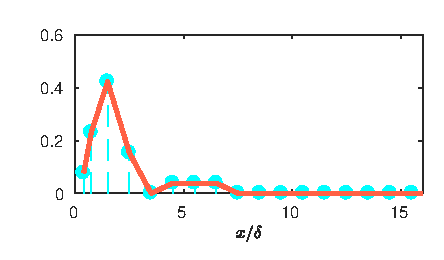
\includegraphics[width=3.0in,height=1.5in]{chnl_stDist_h_33_mode_3_std_0d50}}
		\put(3.0,0){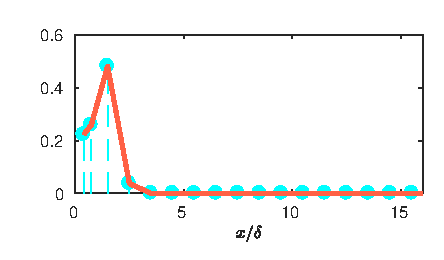
\includegraphics[width=3.0in,height=1.5in]{chnl_stDist_h_33_mode_4_std_0d50}}
		\put(0,1.5){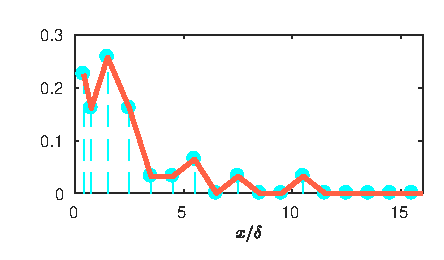
\includegraphics[width=3.0in,height=1.5in]{chnl_stDist_h_33_mode_1_std_0d50}}
		\put(3.0,1.5){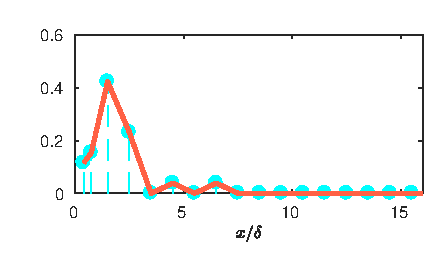
\includegraphics[width=3.0in,height=1.5in]{chnl_stDist_h_33_mode_2_std_0d50}}
		\put(-0.1,2.5){$\mathbf{(a)}$}
		%\put(1.5,0.00){\colorbox{white}{\makebox(0.5,0.05){$\mathbf{x/\delta}$}}}
		%\put(4.5,0.00){\colorbox{white}{\makebox(0.5,0.05){$\mathbf{x/\delta}$}}}
		%\put(-.05,0.60){\colorbox{white}{\makebox(0.2,0.25){$\mathbf{y/\delta}$}}}
		%\put(-.05,2.2){\colorbox{white}{\makebox(0.2,0.25){$\mathbf{y/\delta}$}}}
	  \end{picture}
	\end{minipage}
	\begin{minipage}{\textwidth}
	\setlength{\unitlength}{1in}
	\begin{picture}(6,3)
		\put(0.2,0){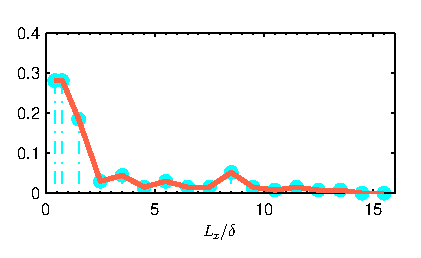
\includegraphics[width=2.87in,height=1.5in]{ek02_stDist_h_24_mode_3_std_0d50}}
		\put(3.2,0){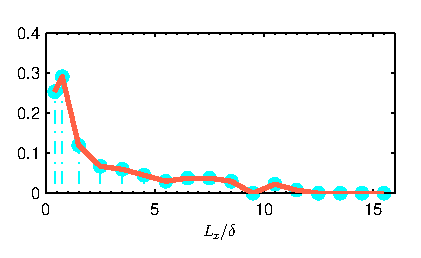
\includegraphics[width=2.87in,height=1.5in]{ek02_stDist_h_24_mode_4_std_0d50}}
		\put(0.2,1.5){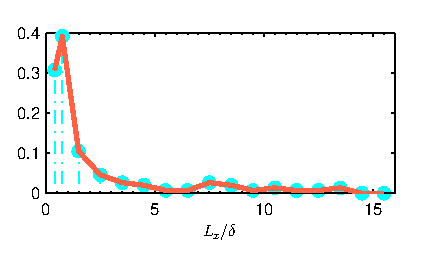
\includegraphics[width=2.87in,height=1.5in]{ek02_stDist_h_24_mode_1_std_0d50}}
		\put(3.2,1.5){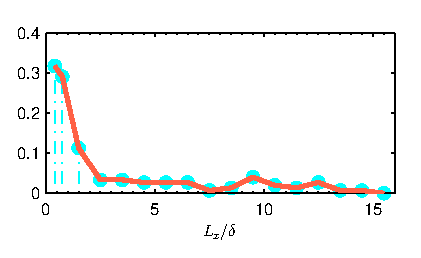
\includegraphics[width=2.87in,height=1.5in]{ek02_stDist_h_24_mode_2_std_0d50}}
		\put(-0.1,2.5){$\mathbf{(b)}$}
		%\put(1.5,0.00){\colorbox{white}{\makebox(0.5,0.05){$\mathbf{x/\delta}$}}}
		%\put(4.5,0.00){\colorbox{white}{\makebox(0.5,0.05){$\mathbf{x/\delta}$}}}		
		%\put(-.05,0.60){\colorbox{white}{\makebox(0.2,0.25){$\mathbf{y/\delta}$}}}
		%\put(-.05,2.2){\colorbox{white}{\makebox(0.2,0.25){$\mathbf{y/\delta}$}}}		
	\end{picture}
	\end{minipage}
\caption{Normalized histogram of the length scales of structures detected in the velocity field reconstructed from individual DMD modes. $x$-axis represents the length scales of structures normalized by the boundary layer depth $\delta$. A discrete set of structures of length scales $ \{ 0.3, 0.5, 1, 2 , 3, 4, 5, 6, 7, 8, 9, 10, 11, 12, 13, 14, 15 \} \delta$ were searched in the velocity field. Subfigures (a) and (b) represents respectively, $CHNL$ and  $EK02$. For each of these two cases the four analysed DMD modes correspond to the first four modes as listed in Table \ref{tab:dmd_freq_chnl} (at $0.5\delta$), and \ref{tab:dmd_freq_ek02} (at $0.48\delta$) and are plotted in clockwise fashion beginning from the top left panel of each subfigure.}	
\label{fig:dmd_length_scale_dist}
\end{figure}
